\subsection{Monotonic-reads consistency}\label{mr:monotonic-reads-consistency}

\subsubsection{Definition}\label{mr:definition}

Monotonic-reads (MR) consistency guarantees that once a client has read a version of a data item, its subsequent reads of that item return the same version or a newer one. For example, suppose a client reads \(x=2\) from one replica and then reads \(x\) through another replica. If the second read returns the same or a newer version, MR is preserved. If it returns an older version, such as \(x=1\), the client observes a step backwards, constituting an MR violation.

\subsubsection{Experimental Design}\label{mr:experimental-design}

Monotonic reads require a client's later read of an item to return a version at least as recent as one it has already observed. The experiment creates a controlled opportunity for a client to observe a new value through one coordinator and subsequently observe an older value through another.

Each iteration uses a separate key. Under the normal topology, a `seed\_write' first stores value 1 using CL = ALL, establishing a common initial state across all three replicas. An update then writes value 2 through node 1 using the selected write consistency level (which can be chosen from ONE, QUORUM and ALL). After the update returns, the client performs two sequential reads: first through node 1 and then through node 2, both at the selected read consistency level. No artificial client sleep is added by the sweep.

The `seed\_write' is an experimental setup, not the write consistency level under investigation. It makes stale reads observable as value 1 instead of relying on an initially absent row. Moving between coordinators represents a client whose requests are redirected by load balancing or reconnection. The table below shows different `seed\_write' CLs and read paths under three different topologies.

{
\begin{table}[H]
\centering
\small
\renewcommand{\arraystretch}{1.15}
\caption{MR setup consistency levels and coordinator paths by topology.}\label{tab:mr-1}
\begin{tabular}{@{}llll@{}}
\toprule\noalign{}
Scenario & Seed\_wrtie CL & Write coordinator & Read path \\
\midrule\noalign{}
normal & ALL & node1 & node1 →node2 \\
partition majority & QUORUM & node1 & node1 →node2 \\
partition minority & ONE & node3 & node3 →node3 \\
\bottomrule
\end{tabular}
\end{table}
}

\subsubsection{Principle and Key Implementation}\label{mr:principle-and-key-implementation}

The experiment can be expressed as follows:

\begin{figure}[H]
\centering
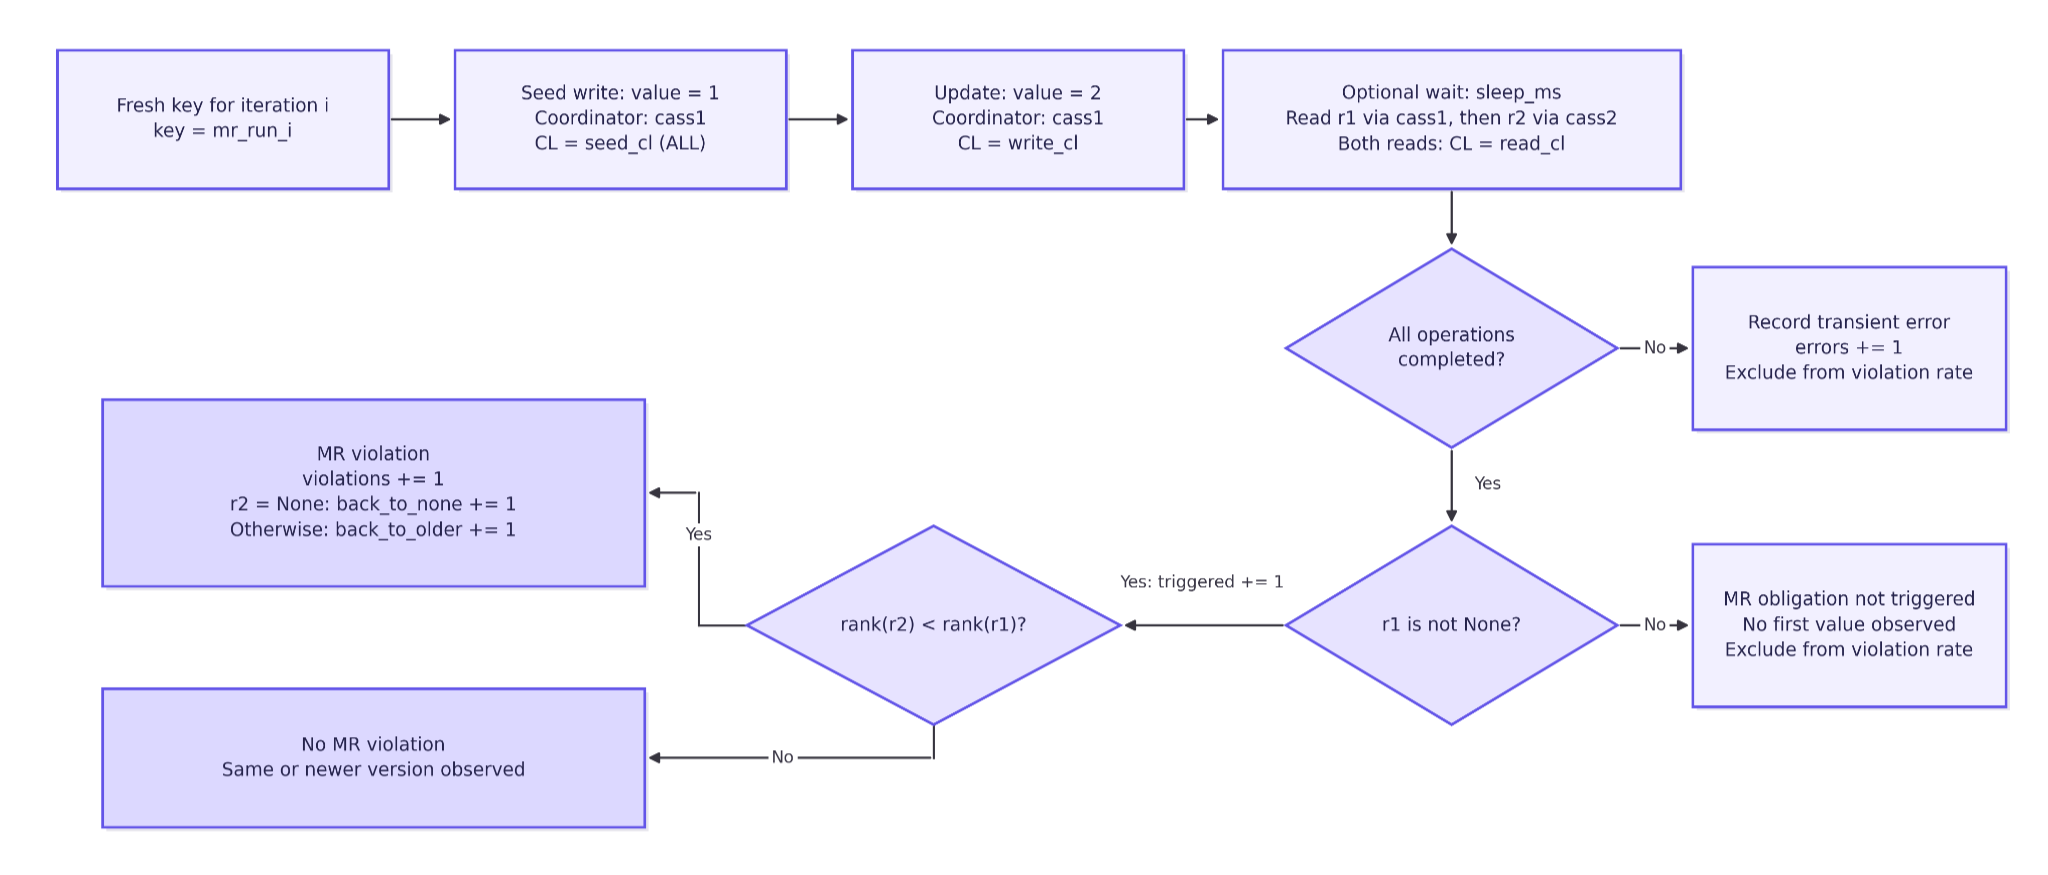
\includegraphics[width=\linewidth]{figures/mr_flow.png}
\caption{Monotonic-reads experimental workflow.}
\label{fig:mr-flow}
\end{figure}

The actual predicate is rank(r2) \textless{} rank(r1), where missing values have rank −1. Since the controlled values are version markers 1 and 2, a transition from 2 to 1 is a monotonic-read violation. Two reads returning 1 are stale relative to the update, but are not a monotonic-read violation: the client has not moved backwards.

For the completed update in this workload, write/read intersection provides a useful sufficient condition: W + R \textgreater{} RF. QUORUM--QUORUM satisfies 2 + 2 \textgreater{} 3, while ALL--ONE satisfies 3 + 1 \textgreater{} 3. This reasoning assumes the intended timestamp order, successful operations, and no competing later writes.

Read repair is relevant to weaker writes followed by quorum reads. Cassandra documents that read\_repair=`NONE' still reconciles returned replica data, but does not repair replicas or provide the general monotonic-quorum-read guarantee associated with blocking read repair. More details can be found here: \href{https://cassandra.apache.org/doc/latest/cassandra/managing/operating/read_repair.html}{Apache Cassandra read-repair documentation}

\subsubsection{Predicted Outcomes}\label{mr:predicted-outcomes}

{
\begin{table}[H]
\centering
\small
\renewcommand{\arraystretch}{1.15}
\caption{Predicted MR outcomes for the tested consistency-level combinations.}\label{tab:mr-2}
\begin{tabular}{@{}
  >{\RaggedRight\arraybackslash}p{(\linewidth - 4\tabcolsep) * \real{0.1600}}
  >{\RaggedRight\arraybackslash}p{(\linewidth - 4\tabcolsep) * \real{0.1600}}
  >{\RaggedRight\arraybackslash}p{(\linewidth - 4\tabcolsep) * \real{0.6800}}@{}}
\toprule\noalign{}
\begin{minipage}[b]{\linewidth}\RaggedRight
Write CL
\end{minipage} & \begin{minipage}[b]{\linewidth}\RaggedRight
Read CL
\end{minipage} & \begin{minipage}[b]{\linewidth}\RaggedRight
Expected Behavior
\end{minipage} \\
\midrule\noalign{}
ONE & ONE & Violations are possible and should become more frequent as delayed propagation outlasts the two client reads. \\
ONE & QUORUM & Violations are theoretically possible, but need not occur in this timing and routing arrangement. \\
QUORUM & QUORUM & No violations expected after the update succeeds, because each quorum intersects its acknowledgement set. \\
ALL & ONE & No violations expected after the update succeeds, because all replicas have acknowledged it. \\
\bottomrule
\end{tabular}
\end{table}
}

In particular, ONE--QUORUM does not satisfy strict write/read intersection: 1 + 2 = 3. If only replica A has value 2, a read involving A can return 2, while a later read involving only B and C can return 1 before propagation reaches them. This is a possible execution, not a prediction of a fixed violation probability. Replica selection should not be assumed uniformly random.

\subsubsection{Results and Analysis}\label{mr:actual-results-and-analysis}

\begin{figure}[H]
\centering
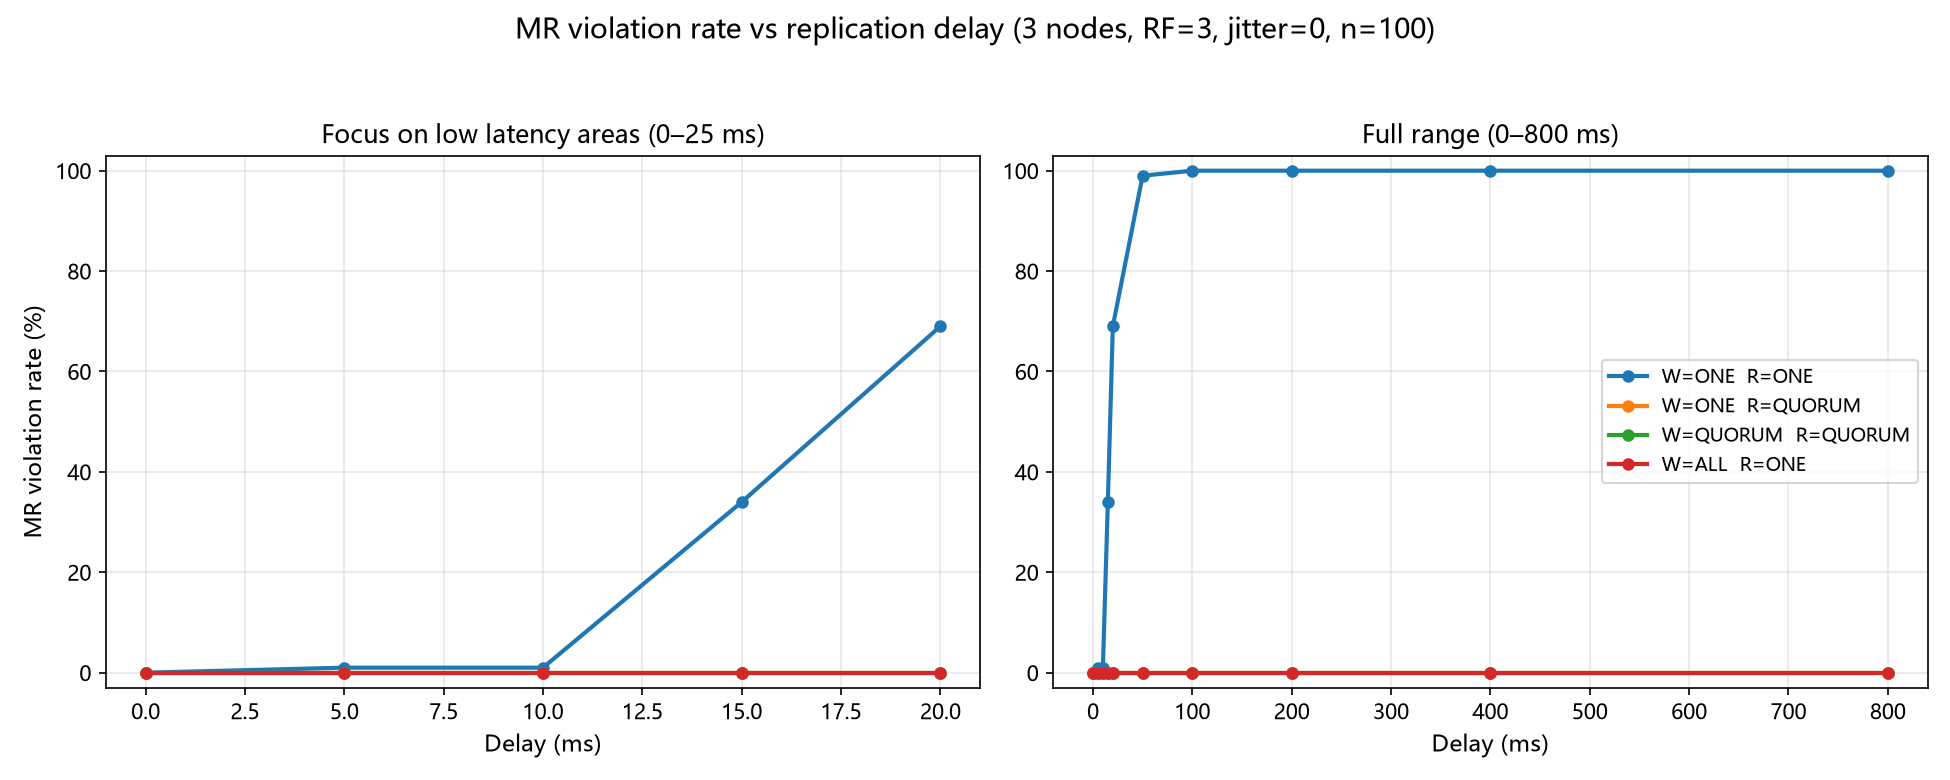
\includegraphics[width=\linewidth]{figures/mr_delay.png}
\caption{Monotonic-reads violation rate versus replication delay.}
\label{fig:mr-delay}
\end{figure}

The above plots demonstrate the violation rates vs different replication delays under different write consistency levels and read consistency levels. Detailed records and original data can be found in \href{https://github.com/LuweiChenbot/Cassandra-Lab/blob/main/results/mr_windows.csv}{monotonic-reads-results}. It is obvious that `ONE--ONE' exhibits a sharp increase between 10 and 50 ms and reaches 100\% at every tested delay of at least 100 ms. The remaining combinations have no observed violations throughout the whole delay range.

The partition rows in the \href{https://github.com/LuweiChenbot/Cassandra-Lab/blob/main/results/mr_windows.csv}{mr results} provide separate availability evidence. When node 3 is isolated and requests use nodes 1 and 2, ONE--ONE records 91/100 violations at delay = 100 ms and jitter = 50 ms; ONE--QUORUM and QUORUM--QUORUM record none. ALL--ONE has 100 operation errors and no valid samples. In the partition-labelled zero-delay run, the three available combinations record no violations, while ALL--ONE again fails every iteration. On the isolated node 3, only ONE--ONE completes the MR experiment, with no violations; combinations requiring a quorum or all replicas have no valid samples.

The ONE--ONE curve is consistent with a race between replica propagation and the client's read sequence. At short delays, the remote replica often receives the update before the second read. As the delay grows, the interval during which replicas hold different versions becomes longer, making a 2-to-1 observation more likely. The observed transition around 15--20 ms is specific to this environment and workload; it is not an intrinsic Cassandra threshold. Zero configured jitter also does not eliminate scheduling, processing, or transport variability.

The absence of ONE--QUORUM violations does not establish a consistency guarantee. A plausible explanation is that the first quorum read introduces an internode exchange, giving the outstanding write time to propagate before the second read. Replica selection and reconciliation can further reduce the opportunity to observe an older version. Because the same delay filter affects internode read traffic, increasing the configured delay can lengthen both propagation and the first read. These mechanisms are interpretations of the setup, not confirmed request-level traces. The supplied aggregate CSV cannot identify the exact replicas or message ordering responsible for the zero rate.

QUORUM--QUORUM and ALL--ONE match the expected intersection argument for this successful-write workload. Their stronger acknowledgement requirements prevent the particular stale-read sequence that ONE--ONE exposes. The partition results additionally show the availability cost: operations requiring unreachable replicas fail. Such failures must not be reported as successful consistency outcomes. Likewise, the isolated-node ONE--ONE result tests a single-node path, not migration between divergent replicas.

\paragraph{Detailed Results Across Topologies}\label{mr:detailed-results-across-topologies}

Each table entry below gives violations / valid iterations; iteration error rate. Every configuration was attempted 100 times. Unlike the plot, these tables include unavailable configurations.

{
\begin{table}[H]
\centering
\small
\renewcommand{\arraystretch}{1.15}
\caption{MR results across topologies: violations / valid iterations; iteration error rate.}\label{tab:mr-3}
\begin{tabular}{@{}
  >{\RaggedRight\arraybackslash}p{(\linewidth - 10\tabcolsep) * \real{0.1667}}
  >{\RaggedRight\arraybackslash}p{(\linewidth - 10\tabcolsep) * \real{0.1667}}
  >{\RaggedRight\arraybackslash}p{(\linewidth - 10\tabcolsep) * \real{0.1667}}
  >{\RaggedRight\arraybackslash}p{(\linewidth - 10\tabcolsep) * \real{0.1667}}
  >{\RaggedRight\arraybackslash}p{(\linewidth - 10\tabcolsep) * \real{0.1667}}
  >{\RaggedRight\arraybackslash}p{(\linewidth - 10\tabcolsep) * \real{0.1667}}@{}}
\toprule\noalign{}
\begin{minipage}[b]{\linewidth}\RaggedRight
Topology
\end{minipage} & \begin{minipage}[b]{\linewidth}\RaggedRight
Delay/\allowbreak Jitter\_ms
\end{minipage} & \begin{minipage}[b]{\linewidth}\RaggedRight
ONE-ONE
\end{minipage} & \begin{minipage}[b]{\linewidth}\RaggedRight
ONE-QUORUM
\end{minipage} & \begin{minipage}[b]{\linewidth}\RaggedRight
QUORUM-QUORUM
\end{minipage} & \begin{minipage}[b]{\linewidth}\RaggedRight
ALL-ONE
\end{minipage} \\
\midrule\noalign{}
normal, initial baseline & 0/0 & 0/100; 0\% & 0/100; 0\% & 0/100; 0\% & 0/100; 0\% \\
normal & 100/50 & 88/100; 0\% & 0/100; 0\% & 0/100; 0\% & 0/100; 0\% \\
partition majority & 0/0 & 0/100; 0\% & 0/100; 0\% & 0/100; 0\% & N/A; 100\% \\
partition majority & 100/50 & 91/100; 0\% & 0/100; 0\% & 0/100; 0\% & N/A; 100\% \\
partition minority & 0/0 & 0/100; 0\% & N/A; 100\% & N/A; 100\% & N/A; 100\% \\
partition minority & 100/50 & 0/100; 0\% & N/A; 100\% & N/A; 100\% & N/A; 100\% \\
\bottomrule
\end{tabular}
\end{table}
}

Normal topology: with all nodes reachable, all four configurations complete every iteration. At 100/50 ms, ONE--ONE exposes a stale second read in 88 trials. The other configurations have no measured violations. Thus reachability alone does not ensure that a client changing coordinators sees monotonically newer data.

Majority partition: the seed write is reduced to QUORUM so that both reachable replicas can be initialized without requiring node 3. Under ONE--ONE, the update may complete on one majority replica while the other still holds the seed value. The partition therefore does not eliminate the divergence window within the majority: 91\% of trials violate MR at 100/50 ms, compared with 0\% at 0/0 ms.

ONE--QUORUM deserves a different explanation here than in the normal topology. During the stable tested partition, a successful quorum read must obtain both reachable replicas, nodes 1 and 2. There is no alternative successful quorum consisting of two other stale replicas. The completed ONE write is represented on at least one member of this pair, so the read can reconcile against that version. The observed zero rate therefore has a stronger workload-specific explanation than the normal three-node ONE--QUORUM zero. This does not convert ONE--QUORUM into a universal session guarantee during arbitrary membership changes or partition healing.

QUORUM--QUORUM also completes with no violations because both reachable replicas acknowledge the update. ALL--ONE cannot complete its update with node 3 isolated; the observed error rate is 100\%. The 91\% majority result and 88\% normal result differ by only three trials out of 100 each. These runs do not establish that partitioning intrinsically increases MR violations; both demonstrate a large stale-read window under weak consistency.

Minority partition\textbf{:} all MR operations use node 3, and the seed CL is ONE. ONE--ONE can complete locally and records no backwards reads. This outcome is expected for the specific same-node overwrite-and-read sequence. It does not show that node 3 is synchronized with the majority, or that a client migrating between the two sides would preserve MR. Each iteration uses its own key, so these tests also do not measure simultaneous conflicting writes to the same key across both partitions.

For ONE--QUORUM on the minority, the local update can succeed but the quorum read cannot obtain a second response. For QUORUM--QUORUM and ALL--ONE, the selected update CL already requires unreachable replicas. This explains why all three configurations have 100\% iteration errors, while only ONE--ONE produces valid consistency observations.

\paragraph{Additional Delay, Jitter, and Read-Path Probes}\label{mr:additional-delay-jitter-and-read-path-probes}

The following table includes all 11 supplementary MR rows. Every row has zero operation errors, so attempted and valid sample counts coincide.

{
\begin{table}[H]
\centering
\small
\renewcommand{\arraystretch}{1.15}
\caption{Supplementary MR experiments with different delays, jitter, and read paths.}\label{tab:mr-4}
\begin{tabular}{@{}
  >{\RaggedRight\arraybackslash}p{(\linewidth - 8\tabcolsep) * \real{0.2000}}
  >{\RaggedRight\arraybackslash}p{(\linewidth - 8\tabcolsep) * \real{0.2000}}
  >{\RaggedRight\arraybackslash}p{(\linewidth - 8\tabcolsep) * \real{0.2000}}
  >{\RaggedRight\arraybackslash}p{(\linewidth - 8\tabcolsep) * \real{0.2000}}
  >{\RaggedRight\arraybackslash}p{(\linewidth - 8\tabcolsep) * \real{0.2000}}@{}}
\toprule\noalign{}
\begin{minipage}[b]{\linewidth}\RaggedRight
Delay/\allowbreak Jitter\_ms
\end{minipage} & \begin{minipage}[b]{\linewidth}\RaggedRight
W-R
\end{minipage} & \begin{minipage}[b]{\linewidth}\RaggedRight
Read Path
\end{minipage} & \begin{minipage}[b]{\linewidth}\RaggedRight
Violation Rate
\end{minipage} & \begin{minipage}[b]{\linewidth}\RaggedRight
Valid Iterations
\end{minipage} \\
\midrule\noalign{}
10/10 & ONE-QUORUM & 1→2 & 0\% & 200 \\
20/10 & ONE-QUORUM & 1→2 & 0\% & 200 \\
50/50 & ONE-QUORUM & 1→2 & 0\% & 200 \\
50/50 & ONE-QUORUM & 2→2 & 0\% & 200 \\
50/50 & ONE-ONE & 1→2 & 63.5\% & 200 \\
50/50 & ONE-ONE & 2→2 & 0\% & 200 \\
50/50 & ONE-QUORUM & 1→3 & 0\% & 200 \\
50/50 & ONE-ONE & 1→3 & 62.5\% & 200 \\
100/50 & ONE-QUORUM & 1→2 & 0\% & 200 \\
100/50 & ONE-ONE & 1→2 & 93\% & 200 \\
100/50 & ONE-ONE & 2→2 & 0\% & 200 \\
\bottomrule
\end{tabular}
\end{table}
}

Effect of changing the read path: at 50/50 ms, ONE--ONE yields nearly identical rates on paths 1 → 2 and 1 → 3: 63.5\% and 62.5\%. The effect is therefore observed with two different second-read coordinators, rather than only node 2. In contrast, 2 → 2 produces no violations at either 50/50 or 100/50 ms. Reusing the same coordinator removes the explicit coordinator switch that creates the main test's backwards-read opportunity. It does not establish that all reads were fresh: both could return 1 without violating MR. Coordinator pinning also does not prove an identical replica set for every read.

Effect of jitter: at base delay 50 ms, the deterministic 50/0 sweep produces 99/100 violations, whereas the 50/50 path-1 → 2 probe produces 127/200 (63.5\%). At base delay 100 ms, the 100/0 sweep produces 100/100 violations, while separate 100/50 runs produce 88/100 and 186/200 (93\%). A plausible explanation is that variable delay allows some updates to propagate earlier, shortening the stale interval for those trials; other packets are delayed longer. This is an interpretation of observed timing-sensitive outcomes. Different sample sizes and sequentially collected runs prevent a precise causal estimate of jitter's independent effect, and the results do not imply that jitter always improves consistency.

Effect of increasing base delay at fixed jitter: for ONE--ONE on path 1 → 2, increasing base delay from 50 to 100 ms while keeping jitter at 50 ms raises the measured rate from 63.5\% to 93\% in the two 200-trial probes. This agrees with the deterministic sweep's evidence that longer propagation windows increase the chance of a stale second read.

Persistent zero results under quorum reads: all six supplementary ONE--QUORUM runs, totalling 1,200 valid trials across different settings and paths, record zero violations. The supplementary data strengthen the observation that this implementation rarely or never exposes the theoretically permitted ONE--QUORUM anomaly under these tested schedules. They do not identify a formal guarantee. Unlike the majority partition, the normal topology still permits different quorum pairs; response timing, selected replicas, and propagation during the first read remain plausible explanations.

\paragraph{Conclution}\label{mr:conclution}

The combined evidence supports three distinct statements. First, switching read coordinators under ONE--ONE exposes clear backwards reads when propagation is slow. Second, the particular same-coordinator probes and normal ONE--QUORUM runs show no backwards reads, but their zero rates must be interpreted in light of path and timing. Third, partitions change which requests can finish: majority quorums remain available, while the isolated minority can serve only local ONE requests in the MR test.

A single pooled MR percentage would mix these different questions. For example, grouping all partition rows together would combine a majority path with 91\% violations and a minority same-node path with 0\%, as well as configurations producing no valid samples. Reporting them separately preserves both the consistency and availability findings.
